% =====================================================================
% draft.tex — "A New Class of Cellular Automata"
%
% A RESULTS paper, refactored from main.tex (which is an exploration note).
% Joe, 2026-07-17: "I bet we could write a straightforward five-to-ten-page
% paper, including pictures. Rather than 'What Undecidability Feels Like From
% the Inside' I might call it 'A new class of cellular automata'."
%
% WHAT CHANGED, and why. main.tex is 1,197 lines built around a fail bank —
% Joe: "even the fail bank sounds like exploratory data analysis". This keeps
% only what survives as a RESULT and demotes the negatives to the one paragraph
% that explains them.
%
% IN:   the object; the parity theorem; the closed form; fixed-byte counts = 2^k;
%       the census (5x death, monotone in k); the prospective test (reduced
%       rotate+2); bias-not-absorber; the interrupter; and the headline —
%       EVERY FIXED POINT SITS AT LANGTON'S lambda = 1/2, exactly, all 40,320,
%       zero violations, with a two-line proof.
% OUT:  transfer (never shown); the tokamak (cascade 0/12 = identity 0/12, not a
%       win, per lon-claude-6's own control); the duet (MI null); the policy
%       population (blend fired 0.2% of calls); C_mu (a frozen barcode beats
%       Rule 110); the heads (dose 1/80).
% DEMOTED: the three-metric fail bank -> one paragraph. Parity is not a metric
%       property, so distance-geometry cannot see it. That is an explanation,
%       not twenty pages.
% =====================================================================
\documentclass[man,12pt,floatsintext]{apa7}

\usepackage[american]{babel}
\usepackage{csquotes}
\usepackage{amsmath,amssymb}
\usepackage{amsthm}
\usepackage{booktabs}
\usepackage{graphicx}
\usepackage{xcolor}
\usepackage{subcaption}
\usepackage[most]{tcolorbox}
\usepackage{needspace}
\usepackage[style=apa,backend=biber]{biblatex}
\addbibresource{refs.bib}
\usepackage{nameref}

\newcommand{\sig}{\sigma}
\newcommand{\bit}[1]{\mathrm{bit}[#1]}
% Sections are unnumbered in apa7 `man' mode, so \ref{sec:..} is empty;
% cross-reference sections by name instead.
\newcommand{\secref}[1]{\emph{\nameref{#1}}}
\newtheorem{theorem}{Theorem}
\newtheorem{corollary}[theorem]{Corollary}
\newtcolorbox[auto counter]{workedexample}[2][]{%
  enhanced,
  breakable,
  colback=green!6,
  colframe=green!45!black,
  boxrule=0.7pt,
  arc=1.5mm,
  left=2.5mm,
  right=2.5mm,
  top=1.5mm,
  bottom=1.5mm,
  fonttitle=\bfseries,
  title={Worked example~\thetcbcounter: #2},
  #1}

\title{A New Family of Operators on Cellular Automata}
\shorttitle{A New Family of Operators on Cellular Automata}
\author{Joseph Corneli}
\affiliation{}

\abstract{%
We describe a cellular automaton whose cells do not hold states but
\emph{rules}, and an operator that rewrites those rules by acting on the
rule's own truth table: $\bit{\sig(k)} := \lnot\,\bit{k}$ for $\sig$ a
permutation of the eight neighbourhoods. The rule's truth table is itself
an eight-cell automaton whose topology is $\sig$ --- an automaton inside
the automaton --- giving a family of $8! = 40{,}320$ operators that is
finite, exhaustively enumerable, and exactly classified.

The classification is by cycle parity. A fixed point of $P_\sig$
exists if and only if every cycle of $\sig$ is even; the number of such
$\sig$ is $((2n-1)!!)^2$, which for $S_8$ gives $105^2 = 11{,}025$ of
$40{,}320$, or $27.34\%$. In a census of the $20{,}256$ mirror orbits, run
under a spatial rule-field dynamics, the all-even class is observed to go
extinct several times more often than the rest.

The main result concerns where those fixed points \emph{are}. Without
exception, across all $40{,}320$ operators, every fixed point that exists has
exactly four one-bits: a \emph{balanced} truth table, equivalently Langton's
activity $\lambda = 1/2$. This is forced by parity---an alternating colouring
assigns each even cycle of length $2m$ exactly $m$ ones, so the total is
$8/2 = 4$ necessarily. A balance long associated \emph{empirically} with
Langton's edge of chaos is here an exact and elementary consequence of the
fixed-point condition. Operators with all-even cycle structure possess these
fixed points; operators with any odd cycle possess none.

Possessing a fixed point at $\lambda = 1/2$ is not, however, the same as
sustaining complex behaviour: $P_\sig$ is a bijection, so a fixed point is
not by itself an attractor. In the spatial dynamics we run, the all-even
class is observed to settle onto its fixed points more readily---and because
every fixed point shares the one value, $\lambda$ cannot distinguish an
operator whose field stays diverse from one whose field collapses. For that
we use a simple population observable, the count of distinct rules present
over time, which in the runs we report separates the rotations that sustain a
diverse field from those that do not.}

\begin{document}
\maketitle

\section{The Object}
\label{sec:object}

A cellular automaton normally evolves a field of \emph{states} under one
fixed rule. Invert that arrangement: let each cell hold a \emph{rule}, and
let an operator evolve the field of rules. An elementary cellular automaton
(ECA) rule is an eight-bit truth table $\bit{k}$, with $k$ ranging over the
eight three-cell neighbourhoods. We study the operator $P_\sig$, parameterised by a
permutation $\sig \in S_8$ that acts on the rule's own table. Writing a rule
as a map $g\colon \{0,\dots,7\} \to \{0,1\}$, the operator sends $g$ to
$P_\sig g$ defined by
\begin{equation}
(P_\sig\, g)(j) \;=\; \lnot\, g\bigl(\sig^{-1}(j)\bigr),
\qquad\text{equivalently}\qquad \bit{\sig(k)} := \lnot\,\bit{k}.
\label{eq:prop}
\end{equation}
Each output bit is one input bit, at the position $\sig$ moves it to, negated;
$P_\sig$ is thus a permutation of the eight coordinates composed with a global
complement. The truth table is thereby itself an eight-cell automaton whose
wiring is $\sig$ and whose update is Boolean negation --- an automaton inside
the automaton. Equation~\eqref{eq:prop} defines a family of $8! = 40{,}320$
operators that is finite, exhaustively enumerable, and, as we show below,
exactly classified. Box~\ref{box:propagator} works through one member of the
family bit by bit.

\begin{workedexample}[label={box:propagator}]{A propagator by hand}
\small
Write an ECA rule in Wolfram's standard neighbourhood order:
\begin{center}
\setlength{\tabcolsep}{3.2pt}
\begin{tabular}{c@{\quad}*{8}{c}}
neighbourhood & $111$ & $110$ & $101$ & $100$ & $011$ & $010$ & $001$ & $000$ \\
\midrule
Rule 110 & $0$ & $1$ & $1$ & $0$ & $1$ & $1$ & $1$ & $0$ \\
\end{tabular}
\end{center}
Thus Rule~110 is the byte $01101110$. Let $\sig(k)=k+2\pmod 8$:
each source bit is complemented and written two positions further along.
Carrying out the eight writes gives
\[
P_{+2}(01101110)=01100100,
\]
which is Rule~100. This changes what the cell does to its black-and-white
phenotype. For example, neighbourhood $011$ maps to $1$ under Rule~110 but
to $0$ under Rule~100. The propagator has not directly flipped a phenotype
cell; it has changed the truth table that the cell will use.
\end{workedexample}

The bare operator acts on one eight-bit rule. In the spatial experiments it
is placed inside a two-layer cellular automaton: a field of rules (the
\emph{genotype}) governs a field of black-and-white states (the
\emph{phenotype}), while neighbouring rules also interact. Box~\ref{box:metaca-step}
spells out one complete local update; this is the computation behind the
space--time diagrams in Figure~\ref{fig:regimes}.

\Needspace{0.72\textheight}
\begin{workedexample}[label={box:metaca-step}]{One site, one complete MetaCA step}
\small
At time $t$, site $x$ holds an eight-bit rule $g_x(t)$ and a phenotype bit
$X_x(t)$. One ordinary propagator step has three parts.
\begin{enumerate}
\item \textbf{Express the current rule.} The phenotype neighbourhood is
evaluated by the rule at its centre:
\[
X_x(t+1)=g_x(t)\bigl(X_{x-1}(t),X_x(t),X_{x+1}(t)\bigr).
\]
\item \textbf{Blend neighbouring rules.} For each truth-table position $j$,
inspect the three genotype bits
$\bigl(g_{x-1}(j),g_x(j),g_{x+1}(j)\bigr)$. If the two outer bits agree, copy
their value. Thus $(0,1,0)$ blends to $0$. If they disagree, the centre rule
decides by treating the triple as one of its ECA neighbourhoods. The eight
coordinate-wise decisions form an intermediate rule
\[
h_x=B\bigl(g_{x-1}(t),g_x(t),g_{x+1}(t)\bigr).
\]
\item \textbf{Propagate the blended rule.} Apply the selected wiring to that
intermediate byte:
\[
g_x(t+1)=P_\sig(h_x).
\]
\end{enumerate}
The ordinary runs apply $P_\sig$ once. The historical Figure~8 accident,
replayed in Figure~\ref{fig:figure8}, applied its off-by-one propagator twice.
\end{workedexample}

The substrate---a cellular automaton whose cells hold rules rather than
states---is not itself new \parencite{corneli2015search}; what we study
is the \emph{operator} of Equation~\eqref{eq:prop}, understood as an
enumerated, exactly classified family. That 2015 paper found a single
member of this family, encountered through a programming error and not
recognised as one of many; we now give the family an essentially complete
characterisation. The canonical symmetry group of ECA
rule space has order four (reflection $\times$ complement, collapsing $256$
rules to $88$ classes) \parencite{svozil2025symmetries}; it is not $S_8$,
and the negation-carrying, $\sig$-parameterised family of
Equation~\eqref{eq:prop} does not appear in it. Rule-space permutation as a
parameterised, enumerated family with a derived fixed-point structure does
not appear in the literature we have surveyed; the nearest neighbours
augment cellular automata with state-dependent feedback
\parencite{pavlic2014selfref} rather than permuting the rule itself. Two
established genres are adjacent but distinct: per-cell rules (non-uniform or
$\nu$-CA \parencite{dennunzio2011nonuniform}) and rules that change during
evolution (rule-changing or programmable CA
\parencite{mori1998rulechanging}). A
referee should note the trap in the first: a $\nu$-CA drawing rules from a
finite set is equivalent to a uniform CA on the product alphabet
\parencite{dennunzio2011nonuniform}, so the substrate is not where novelty
lives. It lives in the fixed-point structure of the operator, which is what
the rest of this paper is about.

\begin{figure}[tp]
\centering
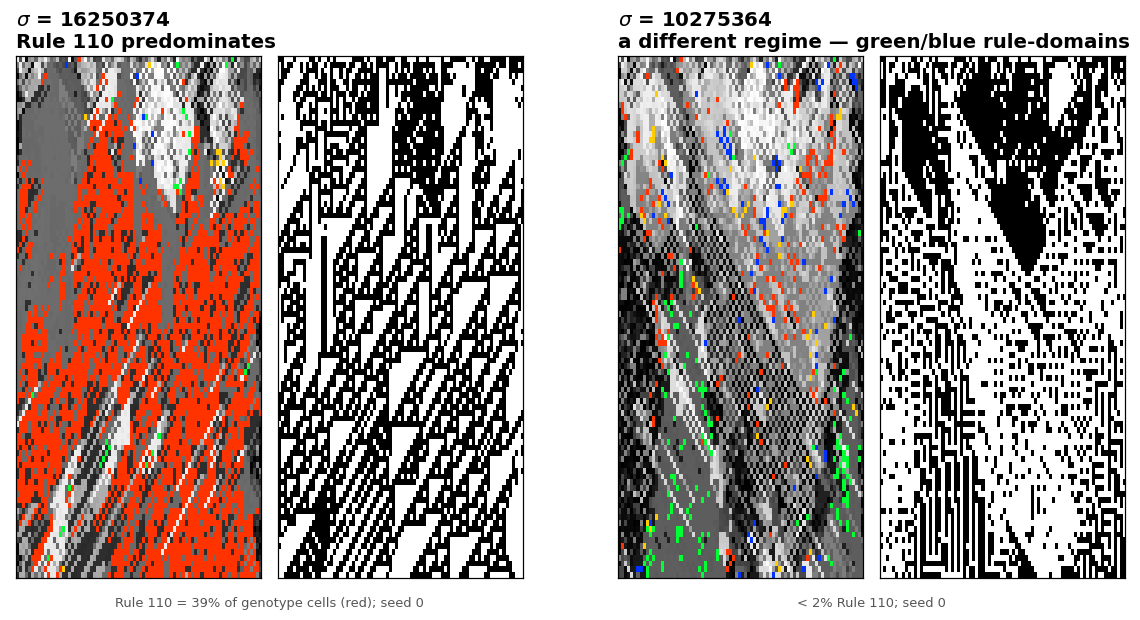
\includegraphics[width=\linewidth]{figures/rule110_spread.png}
\caption{Two operators from the family, each shown over time as genotype
(256-colour, left) and phenotype (black and white, right). Under
$\sig = 16250374$ the genotype field comes to be dominated by ECA
Rule~110---the red cells, $29\%$ of the genotype at the representative seed
($35\%$ over six seeds)---and the phenotype accordingly displays Rule~110's
characteristic gliders; under $\sig = 10275364$ a different regime of
rule-domains forms (green and blue, under $2\%$ Rule~110). The operator does not merely stir rule space: it
drives it toward particular, computationally distinguished rules. Genotype
colours are the legacy engine's own.}
\label{fig:regimes}
\end{figure}

\section{The Classification}
\label{sec:classification}

\subsection{Fixed points exist iff every cycle is even}

\begin{theorem}\label{thm:parity}
$P_\sig$ has a fixed point (a fixed rule) if and only if every cycle of
$\sig$ has even length. Since a one-cycle has odd length, this already
requires $\sig$ to be fixed-point-free.
\end{theorem}

\noindent A fixed rule is a $g$ invariant under~\eqref{eq:prop}, i.e.\ a
$\sig$-equivariant Boolean colouring with $g(\sig k) = \lnot\,g(k)$.
Follow a cycle of length $L$: equivariance forces
$g(k) = (\lnot)^{L} g(k)$, and $(\lnot)^{L}$ is the identity exactly when
$L$ is even; conversely, colour each orbit by the parity of its distance
from a chosen representative. A one-cycle of $\sig$ ($L=1$) is odd and so
admits no such colouring, which is why even cycles are required throughout.

Box~\ref{box:even-cycle} shows the theorem on the offset-$+2$ operator. The
same small calculation also makes the later $2^k$ count and forced
$\lambda=1/2$ balance visible before we state them generally.

\begin{workedexample}[label={box:even-cycle}]{Why even cycles work}
\small
For offset $+2$ on eight truth-table positions,
\[
\sig=(0\;2\;4\;6)(1\;3\;5\;7).
\]
A fixed rule must change colour at every arrow because
$g(\sig k)=\lnot g(k)$. Around either four-cycle it can therefore read
$0101$ or $1010$: after four negations it returns consistently to its
starting bit. The two cycles can be chosen independently, giving
\[
2^2=4\quad\text{fixed rules:}\quad
51,\ 102,\ 153,\ 204.
\]
Each contains four zero-bits and four one-bits. An odd cycle fails for the
same elementary reason: after an odd number of negations it returns to the
starting position demanding the opposite of the bit with which it began.
\end{workedexample}

This is the signed-cycle fixed-point theorem of Boolean-network theory
\parencite{aracena2008maximum} specialised to~\eqref{eq:prop}: our operator
is a Boolean network whose signed interaction digraph is $\sig$ with every
arc negative, a negation-cycle of length $\ell$ has sign $(-1)^\ell$, and
an isolated negative cycle admits no fixed point while a positive (even)
one admits exactly two. We contribute a machine-checked proof of the
specialised statement in Lean~4 / Mathlib.\footnote{%
\texttt{DarkTower/Patterns/Propagator.lean}, theorem
\texttt{hasAlternatingColouring\_iff\_cycleType\_even}; \texttt{lake build}
clean, no \texttt{sorry} or \texttt{axiom}.}

\subsection{The closed form}

The number of $\sig \in S_{2n}$ with all cycles even is $((2n-1)!!)^2$, with
exponential generating function $\sum_n ((2n-1)!!)^2 x^{2n}/(2n)! =
1/\sqrt{1-x^2}$ (the ``set of even cycles'' construction).
For $S_8$ this is $105^2 = 11{,}025$ of $40{,}320$, or $27.34\%$. The count
is classical: it is \textcite{oeis_a001818} and appears as
\textcite[Problem~5.34(c)]{stanley1999enumerative} and in
\textcite{riordan1968combinatorial}. We claim it only as the enumeration of
our operator family, not as a new identity.

\subsection{Fixed bytes number $2^k$}

An all-even $\sig$ with $k$ cycles has exactly $2^k$ fixed bytes; any
$\sig$ with an odd cycle has none. Each even cycle admits exactly two
alternating colourings, chosen independently across cycles, whence $2^k$;
the zero case is Theorem~\ref{thm:parity}. This too is machine-checked.%
\footnote{\texttt{alternatingColouring\_card\_eq\_two\_pow\_cycleType\_card}.}
Summed against these weights the family is consistent:
$\sum 2^{k}$ over all-even $\sig$ equals $(2n)! = 8! = 40{,}320$, the total
number of fixed bytes across the family.

\section{Every Fixed Point Is Balanced}
\label{sec:lambda}

Langton's $\lambda$ measures a rule's \emph{activity}: the fraction of its
neighbourhood entries that map to the non-quiescent
state~\parencite{langton1990computation}. For an eight-bit ECA table it is
the Hamming weight over eight, $\lambda = \lVert r \rVert_1 / 8$, running
from $0$ (every neighbourhood dies) through $1/2$ to $1$. Langton's thesis
was that complex, computation-supporting behaviour concentrates near a
critical value of $\lambda$. That transition was demonstrated most clearly
for larger rule tables (notably $K=4$, $N=5$); for the two-symbol,
three-neighbour case of the ECAs, Langton is explicit that $\lambda$ is only
roughly correlated with dynamical behaviour, and later work is cautious about
the correlation \parencite{mitchell1993revisiting}. Our theorem below is
about the value $\lambda = 1/2$ itself---\emph{balance}, a property of the
truth table---and we keep that exact statement separate from the empirical
edge-of-chaos programme it evokes.

\subsection{Every fixed point has $\lambda = 1/2$}

\begin{theorem}\label{thm:lambda}
Every fixed point of every operator in the family has exactly four one-bits;
equivalently, Langton's activity parameter $\lambda = 4/8 = 1/2$.
\end{theorem}

\noindent By Theorem~\ref{thm:parity} each cycle has even length $2m$; an
alternating colouring assigns such a cycle exactly $m$ ones; summing over
cycles gives $(\sum L)/2 = 8/2 = 4$. Exhaustive enumeration confirms it:
across all $40{,}320$ operators and all their fixed points, every one has
Hamming weight four, with zero exceptions. The statement is machine-checked
for $\mathrm{Fin}\,8$.\footnote{%
\texttt{alternatingColouring\_true\_card\_eq\_four}: the true-cells and
false-cells are put in bijection by $\sig$, forcing each to number four.}

We are deliberate about the standing of this result. Langton's critical
value was obtained empirically, as a statistic over rule space
\parencite{langton1990computation}, and its status as an order parameter
was contested: \textcite{mitchell1993revisiting} refuted
\textcite{packard1988adaptation}'s specific genetic-algorithm clustering
claim, not the definition of $\lambda$, which survived as one axis among
others such as Wuensche's $Z$ \parencite{wuensche1999classifying}. There is
a folklore intuition for why $1/2$ is special --- binomial sampling variance
$\lambda(1-\lambda)$ is maximal there --- and it is not ours; and it has been
noted that $\lambda$ alone does not fix a rule's dynamical class, distinct
classes coexisting at a single value \parencite{sakai2002edge}. What
Theorem~\ref{thm:lambda} adds is narrower and firmer than any of these: under
the complementation in~\eqref{eq:prop} the value $1/2$ is \emph{forced} as an
algebraic matter, because any alternation-under-complement colouring is
balanced by parity. We claim balance, exactly; the connection of balance to
edge-of-chaos dynamics we treat as interpretation, not as part of the
theorem.

\subsection{The cast: which rules survive, and how many}

Under an all-even $\sig$, the fixed points of $P_\sig$---the rules it maps to
themselves---number $2^k$, where $k$ is the number of cycles of $\sig$
(\secref{sec:classification}): each even cycle admits two alternating
colourings, chosen independently across cycles. In the spatial runs these are
the rules onto which the field is observed to settle. Every one has
$\lambda = 1/2$ (Theorem~\ref{thm:lambda}), so the observed terminal
population is a cast of \emph{distinct} rules---distinct truth tables---sharing
a \emph{single} activity.

The smallest nontrivial case of the count is a single cycle, $k = 1$: two
survivors. The 2015 paper's Figure~8 already exhibited a two-rule residual
(Figure~\ref{fig:figure8}): a random field of tens of distinct rules dies
off to an alternating population of just two, rules $42$ and $170$.
Fittingly, the programming error that produced the family is what pins its
residual at two---the erroneous mutation froze a bit, splitting the field
into the cells that can reach $42$ and those that can reach $170$---so the
phenomenon was on the page before the $2^k$ count explained it.

That die-off curve---the count of distinct rules present over time---is a
natural population-level companion to $\lambda$. Where $\lambda$ is a scalar
assigned to a single rule, this curve is a property of the whole field's
trajectory; and where $\lambda$ is uninformative here---every fixed point
sits at $1/2$---the curve still varies, because it measures the population
rather than the point. We use it cautiously, as an observable rather than an
established order parameter, to tell the rotations whose fields stay diverse
from those whose fields collapse (\secref{sec:interrupter},
Figure~\ref{fig:lambda}).

Diversity of the observed population and singularity of its activity thus
coexist; the metric measures we tried do not separate the two
(\secref{sec:metrics}).

\begin{figure}[t]
\centering
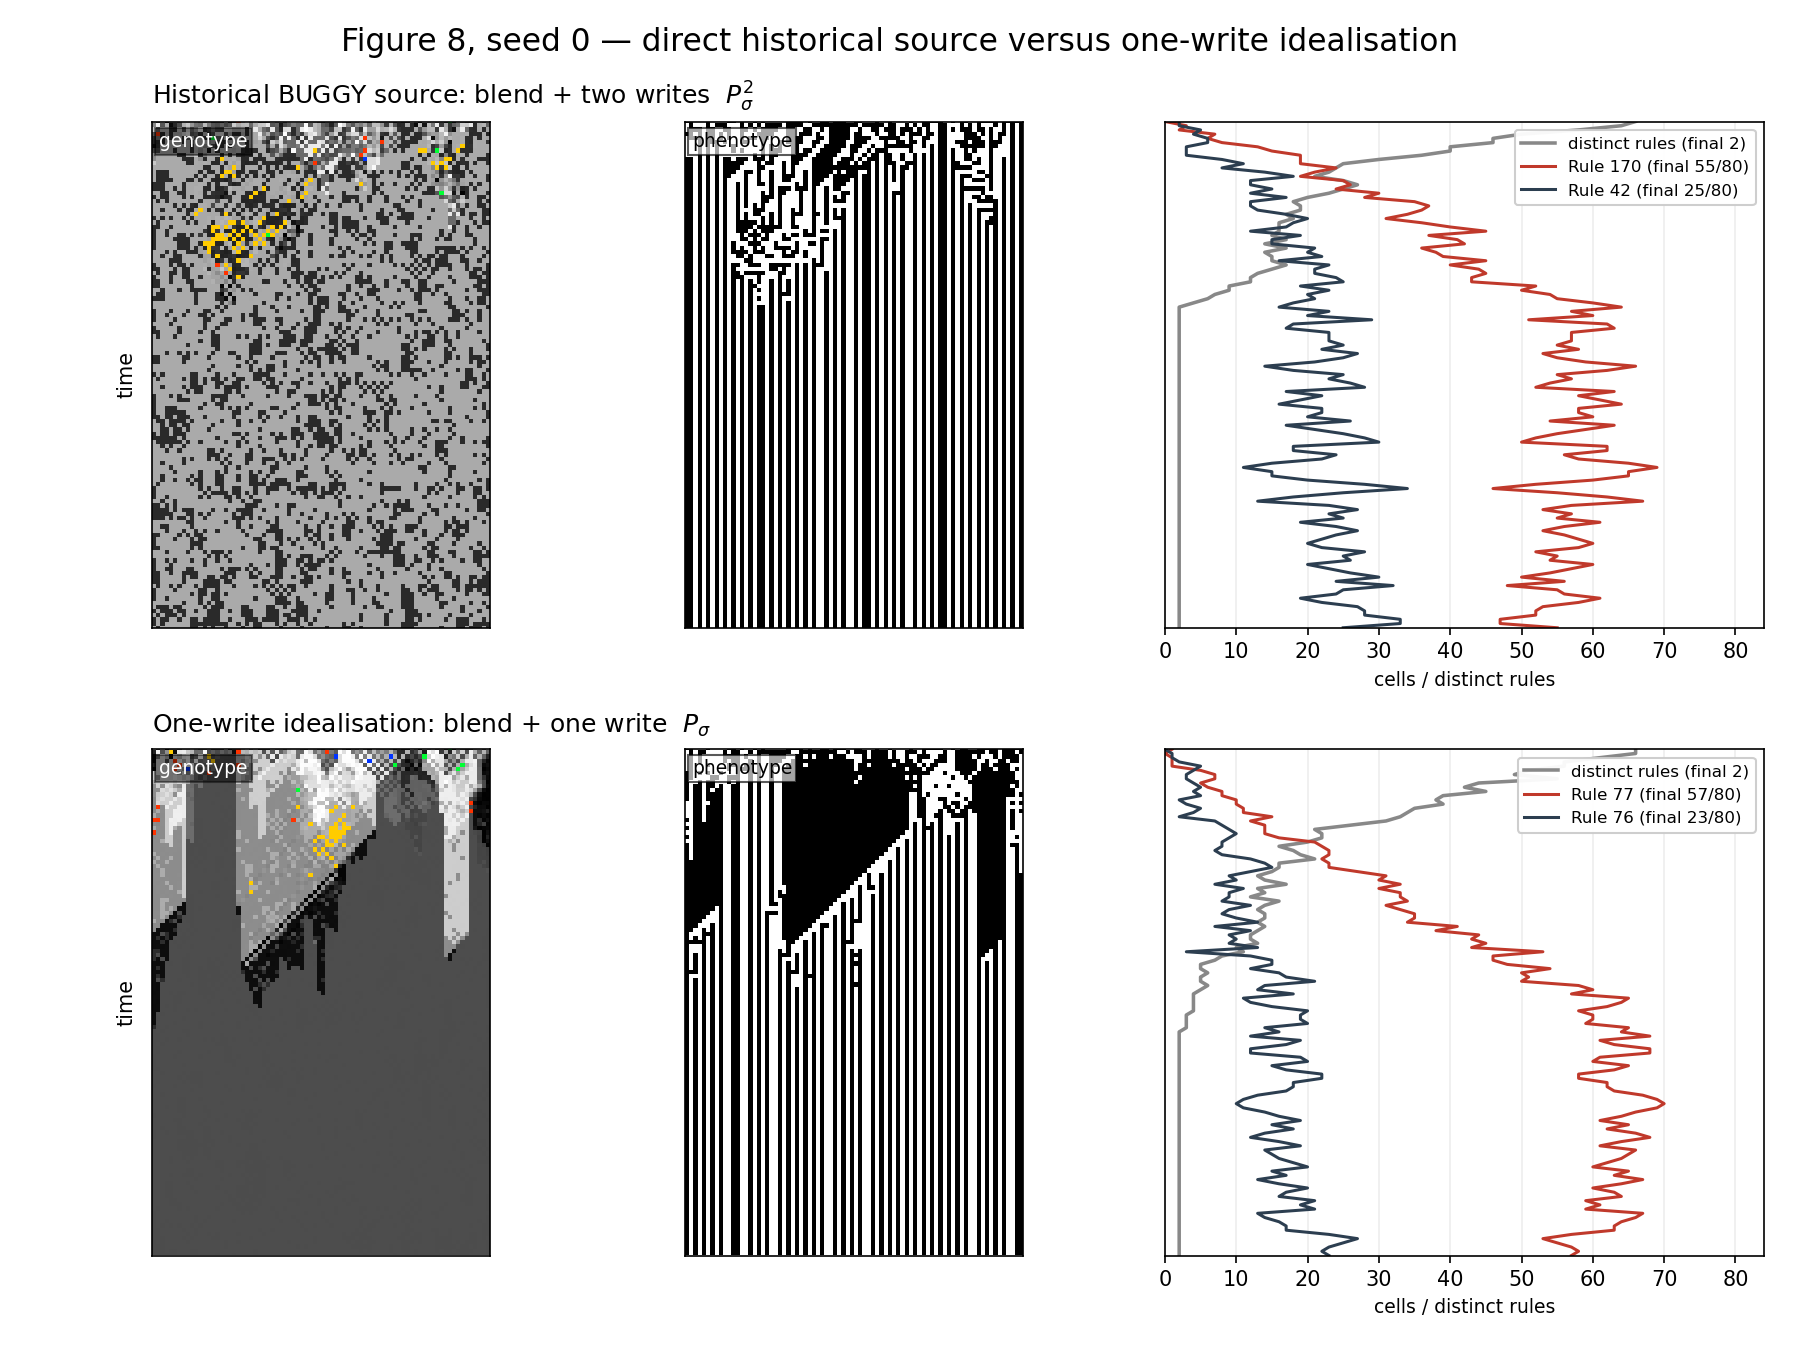
\includegraphics[width=\linewidth]{figures/fig8.png}
\caption{The family's accidental first sighting, separated from its later
idealisation (seed 0, width 80). Top: a direct replay of the historical
Figure~8 source. Its neighbour blend is followed by two independent calls to
the erroneous mutation, equivalently two writes by
$\sigma=[0,0,1,2,3,4,5,6]$. In both rows the distinct-rule count is purple and
dashed. Here it falls from tens to two; rules $170$ (light grey) and $42$ (dark grey) partition the field,
with population traces matching their genotype colours. Bottom: the later
one-write propagator idealisation, which applies the same $\sigma$ only once
after blending. Its terminal genotypes, rules $77$ (red) and $76$ (dark), are
colour-coded to distinguish their adjacent greyscale rule numbers. This lower
panel isolates the propagator cleanly, but is not a
one-for-one reproduction of the 2015 figure. Genotype, phenotype, and
population share the time axis within each row.}
\label{fig:figure8}
\end{figure}

\subsection{A dead genotype can carry a live phenotype}
\label{sec:shell}

The balanced shell is a definite object: exactly $\binom{8}{4} = 70$ rules
carry four active outputs, and by Theorem~\ref{thm:lambda} the absorbing set of
every operator in the family lies wholly inside it. Collapse is therefore not
merely a loss of diversity but a fall onto this particular $70$-rule shell---the
field dies \emph{onto the edge}, at $\lambda = 1/2$, always.

Balance is necessary for a genotype to freeze and silent about what the frozen
rule then does. Run each of the $70$ as an ordinary elementary CA and they
split: $32$ are phenotypically live---sustained change under iteration, the
additive rules $90$, $105$, $150$ and the class-IV rule $54$ among them---while
the rest fall quiescent. The two halves share a single $\lambda$; this is,
inside our family and by construction rather than by survey, the coexistence of
dynamical classes at one activity value that has long been urged against
$\lambda$ as an order parameter \parencite{sakai2002edge}. A field can thus die
in its genotype while the surviving rule keeps its phenotype in motion.

Figure~\ref{fig:shell} is such a field, built to specification. To seat a
collapse on a chosen live rule $R$ it suffices to pair $R$'s four active
positions with its four inactive ones as an involution: four transpositions, an
all-even operator that must collapse (Theorem~\ref{thm:parity}) and that holds
$R$ among its fixed points. Carried out for Rule~$54$ this yields
$\sig = [2\,3\,0\,1\,5\,4\,7\,6]$; run from a random field it drives the
genotype to near-uniformity---two rules survive---while the phenotype never
settles. The field has died onto Rule~$105$, another live tenant of the same
shell, whose additive dynamics keep the black-and-white panel full of
structure. Genotypic death and phenotypic death are not the same event.

One caveat marks the open edge of this. An involution fixes not its target
alone but the whole shell compatible with its pairing, and which tenant a
random field actually reaches is set by the basins, not by the construction: we
aimed at $54$ and the dynamics preferred $105$. Existence is settled---live
survivors are constructible---but \emph{steering} a field onto a named rule is
not, and is the natural next question.

\begin{figure}[t]
\centering
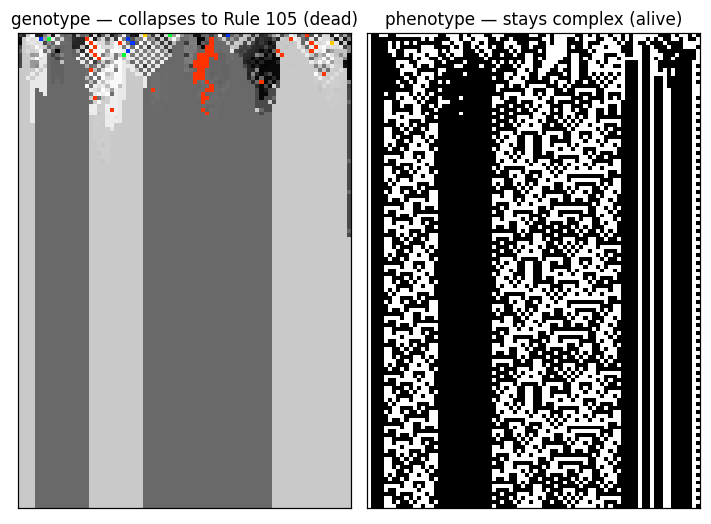
\includegraphics[width=0.82\linewidth]{figures/critical_shell.png}
\caption{A genotypically dead, phenotypically live field. The all-even operator
$\sig = [2\,3\,0\,1\,5\,4\,7\,6]$, built to fix the balanced shell containing
Rule~$105$, collapses the genotype (left, 256-colour) to near-uniformity within
a few dozen rows---two rules survive---yet the phenotype (right) never settles:
the field has died onto Rule~$105$, an additive $\lambda = 1/2$ rule whose
dynamics keep it complex. Seed~$1$, $W = 80$, $T = 120$.}
\label{fig:shell}
\end{figure}

\section{The Census}
\label{sec:census}

\subsection{Parity predicts death across all 20{,}256 orbits}

Theorems~\ref{thm:parity}--\ref{thm:lambda} are statements about fixed
points; we also ran the family as a spatial dynamics to ask whether the
parity dichotomy is reflected in observed behaviour. Reducing the family by
the mirror symmetry gives $20{,}256$ orbits. In our runs---a field of rules
on a one-dimensional lattice, evolved from random initial rules and scored
for extinction of phenotype activity---the all-even class goes extinct
several times more often than the rest, with the tendency increasing in the
number of cycles $k$. We report this as an observed trend, not a measured
law: the present runs fix a single lattice size, boundary condition, initial
distribution, and horizon, and we have not yet tabulated deaths and
denominators by class and by $k$ with seed-level uncertainty---which a
quantitative claim would require. Note also that classifying the enumerated
permutations by cycle parity merely recovers the combinatorial $27.34\%$; the
dynamical content is the \emph{death-rate difference} between the classes, not
the class sizes. Figure~\ref{fig:parity} illustrates the dichotomy with five
representative operators rather than summarising all $20{,}256$.

\begin{figure}[t]
\centering
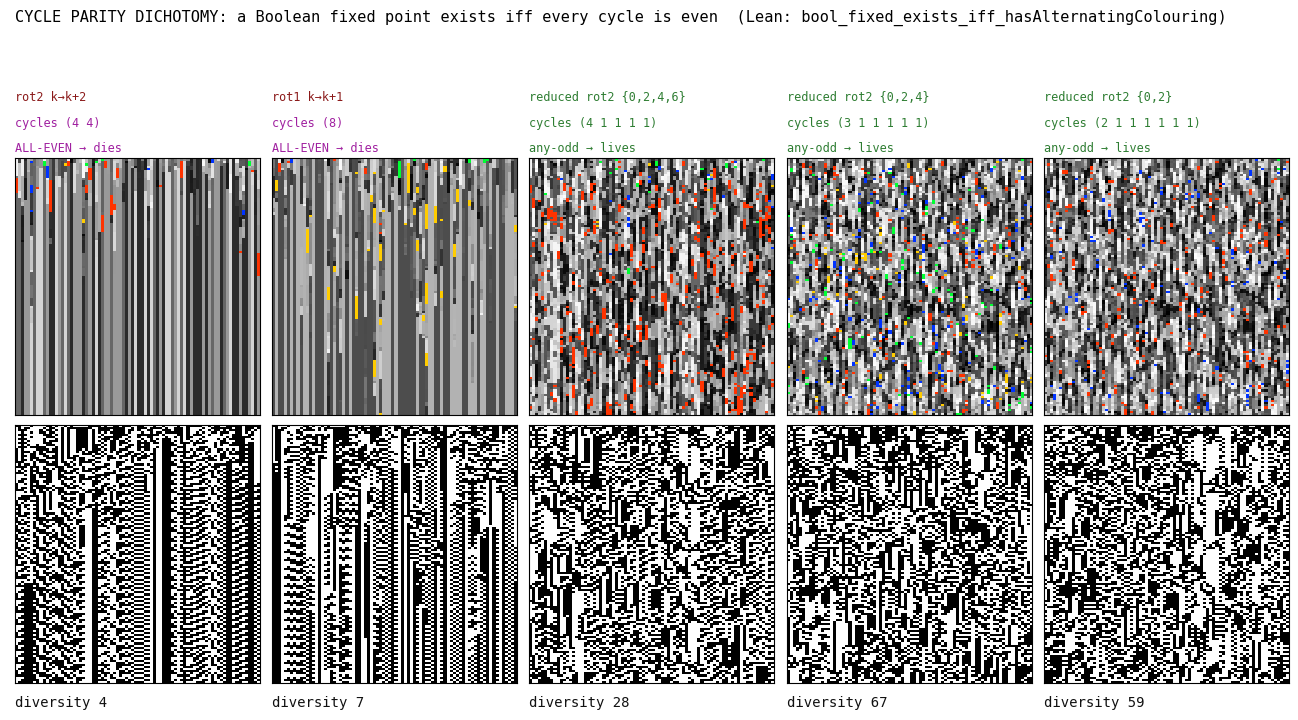
\includegraphics[width=\linewidth]{../../labs/M-aif-tokamak/compositions/parity-dichotomy.png}
\caption{The parity dichotomy, by example (the full census of $20{,}256$
orbits is summarised in the text). Five operators as genotype (top) and
phenotype (bottom) over time. \emph{Left:} the all-even operators
rotate$+2$ and rotate$+1$ possess fixed points (Theorem~\ref{thm:parity})
and, left to settle, the field collapses onto them---rotate$+2$ onto
four rules, its $2^k = 2^2$ count. \emph{Right:} the any-odd operators
(reduced rotate$+2$, acting on a subset so the remaining positions are odd
one-cycles) possess no fixed point, cannot settle, and stay diverse. This
settling is the operator left to itself; a neighbour-blend interrupter
reverses it for the $\gcd 2$ case (Figure~\ref{fig:lambda},
\secref{sec:interrupter}), and that reversal is the dynamical point.}
\label{fig:parity}
\end{figure}

\subsection{A prospective test: reduced rotate$+2$}

To guard against reading structure into a completed enumeration, we fixed a
prediction before running the case. The reduced $\text{rotate}{+}2$
operators act as a single even cycle on a subset of positions and leave the
remaining positions as one-cycles; by that leftover they are \emph{not}
all-even, so by Theorem~\ref{thm:parity} they possess no fixed point and
should fall on the no-fixed-points side of the dichotomy---no rule for the
field to settle onto, and correspondingly less extinction. They do
(Figure~\ref{fig:parity}, right): they stay diverse rather than dying off.
Absence of fixed points forbids settling onto a single rule; it does not
forbid short-period behaviour, and we claim only the observed persistence of
diversity, not literal aperiodicity.

\section{Fixed Points Are Not Attractors}
\label{sec:interrupter}

\begin{figure}[p]
\centering
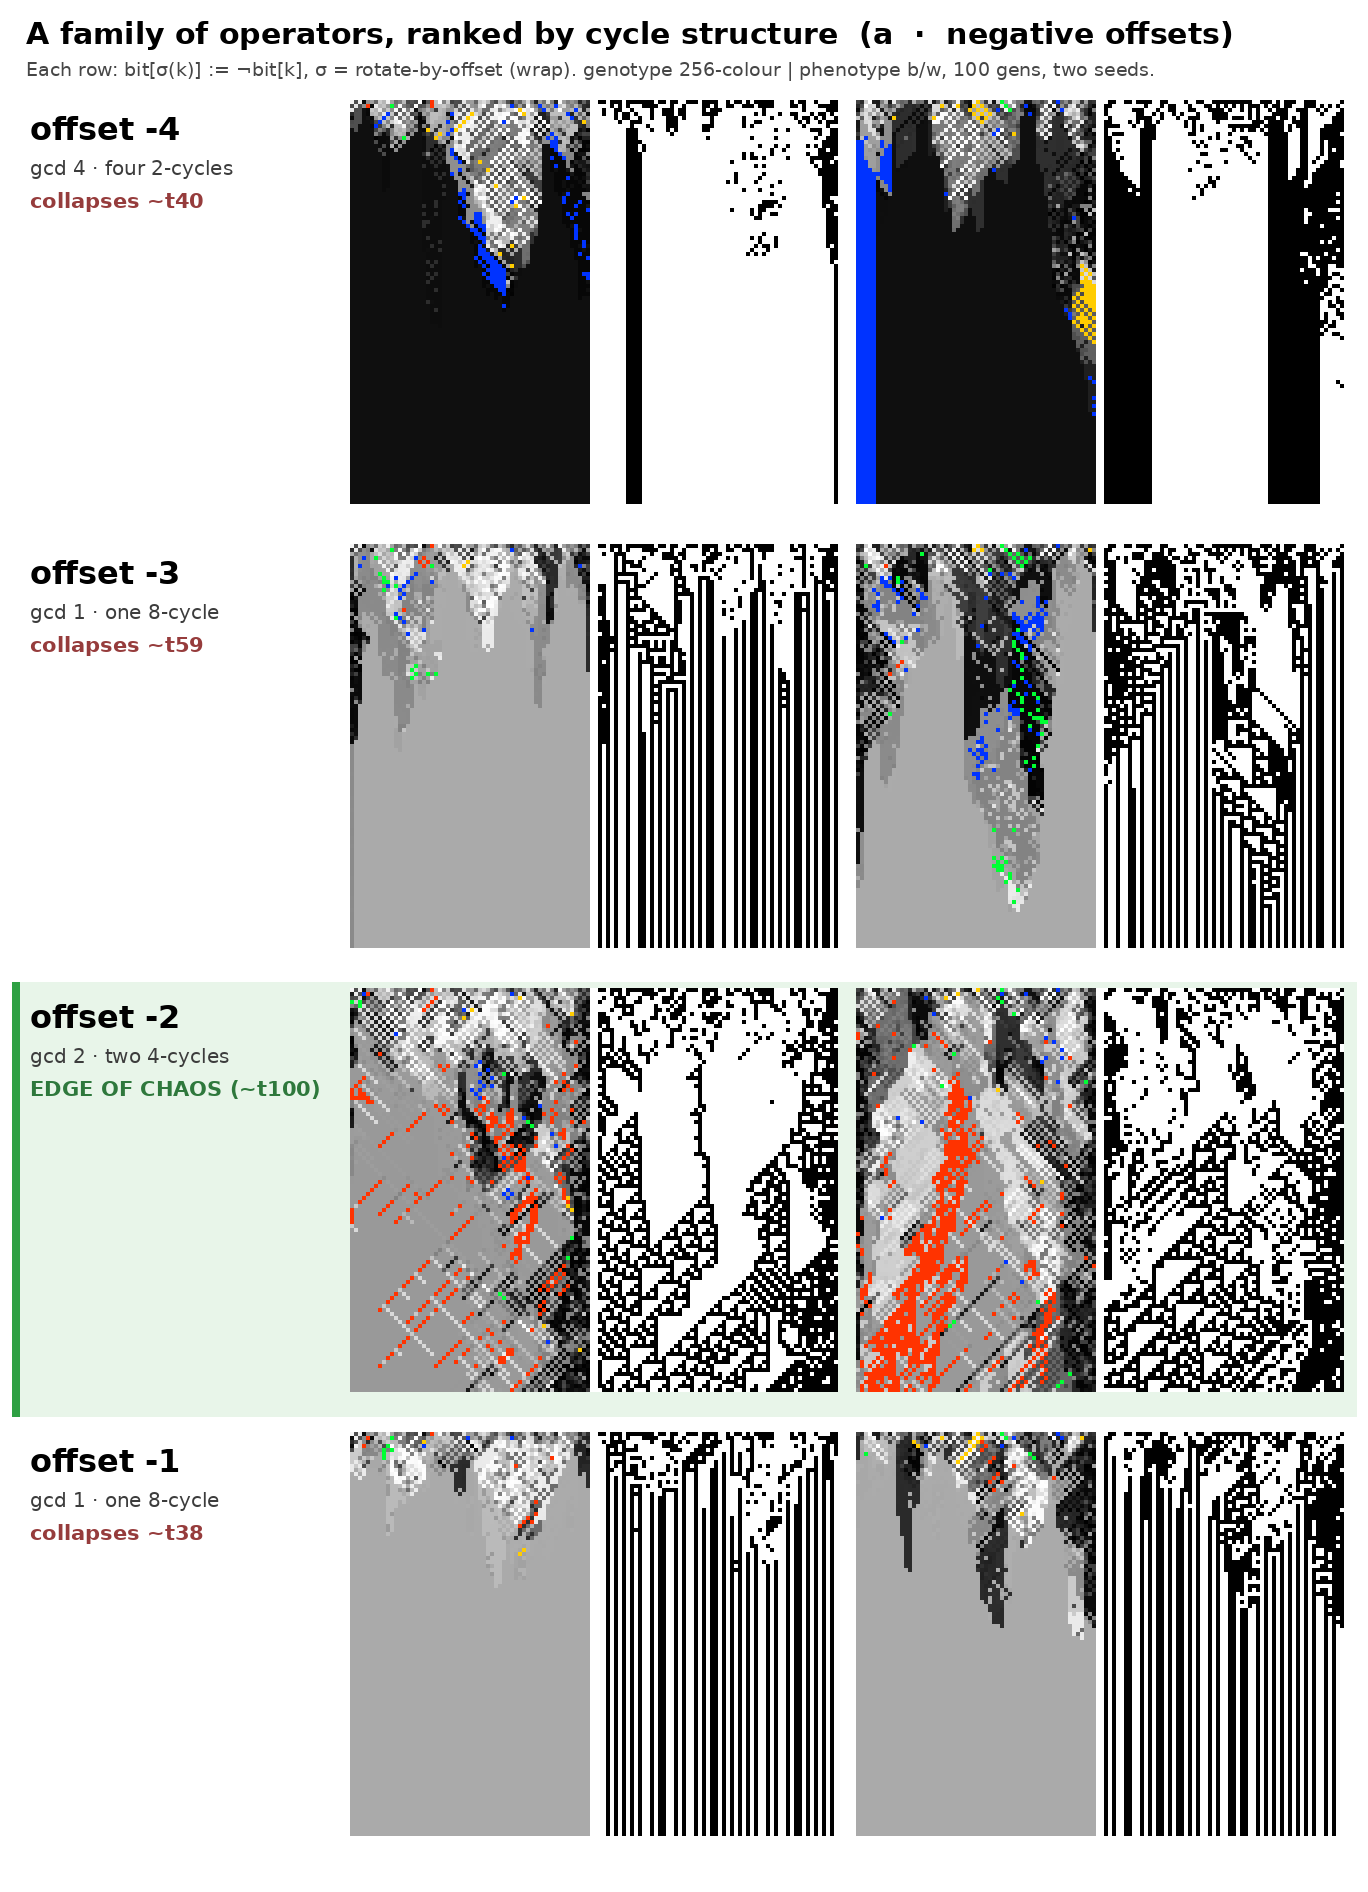
\includegraphics[height=0.92\textheight]{figures/survey_a.png}
\caption{\textbf{(a)~Negative offsets.} The rotation subfamily, ordered by
offset. Each row is one operator $\bit{\sig(k)} := \lnot\,\bit{k}$ with
$\sig$ a wrap rotation, shown for two seeds as genotype (256-colour) and
phenotype (black and white) over the first hundred generations. Every
non-trivial rotation is all-even and so possesses fixed points
(Theorem~\ref{thm:parity}); yet only $\gcd(\text{offset},8)=2$---offset
$\pm 2$, two $4$-cycles, highlighted green---sustains a high-diversity,
visually complex phase. The remaining rotations collapse to near-uniform
fields within a few dozen generations. Continued in panel~(b).}
\label{fig:eoc}
\end{figure}

\begin{figure}[p]
\ContinuedFloat
\centering
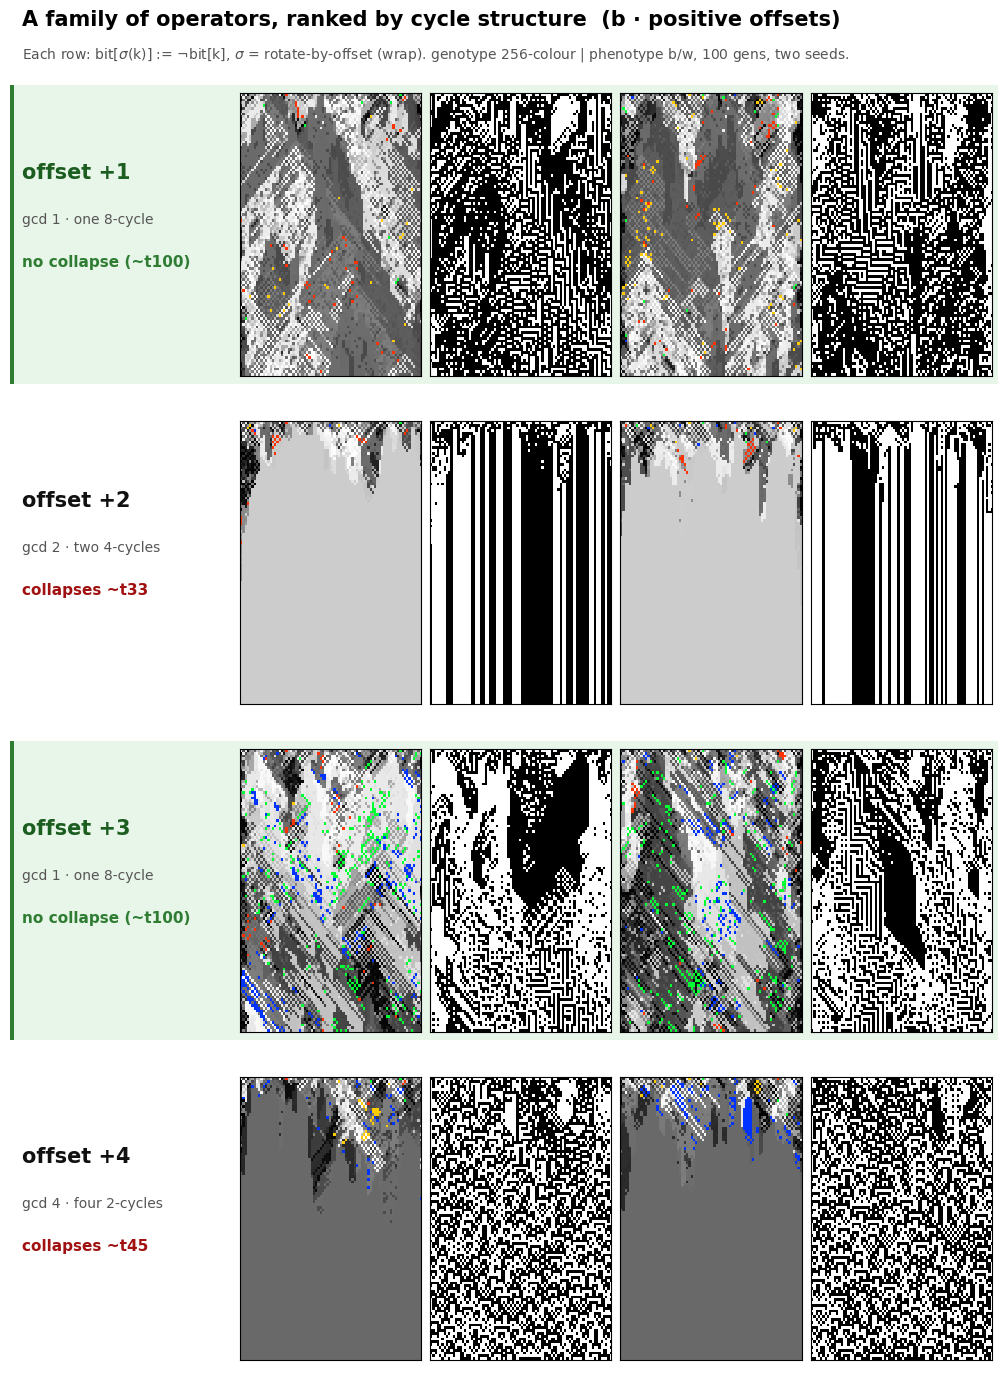
\includegraphics[height=0.92\textheight]{figures/survey_b.png}
\caption{\textbf{(b)~Positive offsets.} Continued from panel~(a). The pattern
is symmetric: offset $+2$ ($\gcd 2$, two $4$-cycles) sustains the
high-diversity phase, the rest collapse. Possessing a fixed point and having
the field stay near it are different properties, and this pair of pages is
the whole paper in one figure.}
\end{figure}

Possessing a fixed point (Theorem~\ref{thm:parity}) is not the same as
reaching one, and $P_\sig$ does not by itself move a rule toward
$\lambda = 1/2$. Because $P_\sig$ complements every bit,
$\lambda(P_\sig g) = 1 - \lambda(g)$: the operator \emph{reflects} activity
across $1/2$, exactly preserving the distance $\lvert\lambda - 1/2\rvert$
rather than contracting toward it. And because $P_\sig$ is a bijection on
bytes, a generic rule lies on a periodic orbit and simply cycles---its fixed
points are fixed, but they are not attractors and have no basins. The only
rules pinned at $\lambda = 1/2$ are the fixed points themselves. Whatever
pull toward balance the \emph{spatial} field exhibits must therefore come
from the coupling between cells and from the interrupter below, not from the
bare map.

The rotation family makes this concrete. Every non-trivial wrap rotation is
all-even and so possesses fixed points (Theorem~\ref{thm:parity}), yet in the
spatial dynamics only offset $\pm 2$---$\gcd(2,8)=2$, two $4$-cycles---sustains
a visually complex, high-diversity field (Figure~\ref{fig:eoc}), persisting to
roughly a hundred generations; the remaining rotations ($\gcd 1$ and
$\gcd 4$) collapse to near-uniform fields within a few dozen. Possessing a
fixed point and having the field stay near it are different properties, and
only the second is visible in a drawing.

This last distinction can be \emph{measured}, with the distinct-rule
population curve as a simple instrument. Every rotation begins at peak
diversity---some seventy distinct rules in a random field---but the
distinct-rule count then diverges sharply by cycle structure
(Figure~\ref{fig:lambda}): offset $\pm 2$ hold around thirty distinct rules
through the longest runs we made ($400$ generations), while every $\gcd 1$
and $\gcd 4$ rotation collapses to one or two within sixty. The persistent
diversity of the $\gcd 2$ operators and the quick collapse of the
rest---visible by eye in Figure~\ref{fig:eoc}---are thus separated by more
than an order of magnitude in this one scalar. We do not claim the count is
an order parameter in the statistical-mechanics sense; it is a useful summary
of what the drawings show, on the two seeds per operator that we ran.

\begin{figure}[t]
\centering
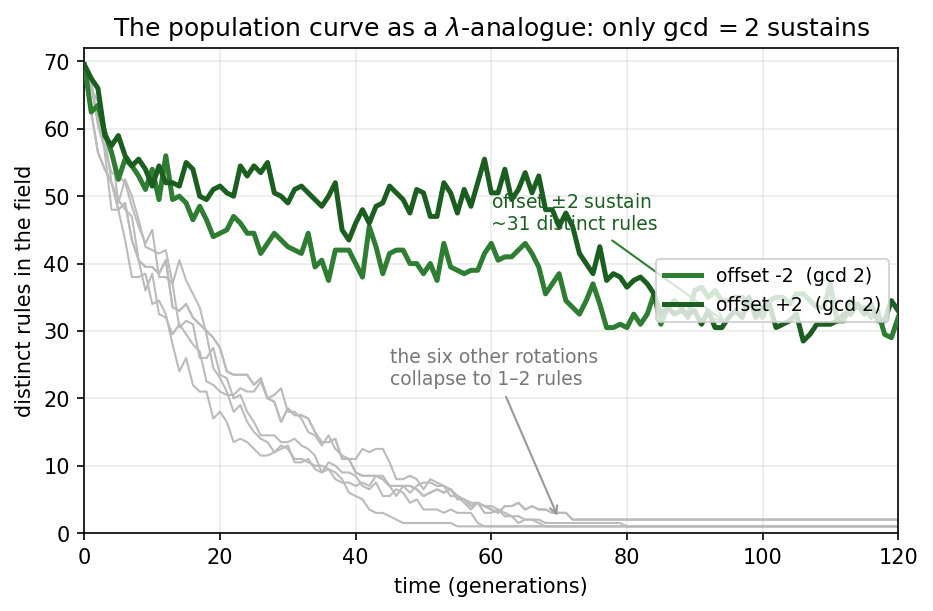
\includegraphics[width=\linewidth]{figures/lambda_analogue.png}
\caption{A population observable: distinct rules in the field over time, for
the eight wrap rotations (two seeds each). All begin at $\approx 70$; only
the two $\gcd 2$ operators, offset $\pm 2$ (green), keep a large diverse
population, while the six others collapse to one or two rules. This makes
quantitative, on the runs shown, the difference visible by eye in
Figure~\ref{fig:eoc}. The interrupting neighbour-blend is essential to the
sustained case: without it these same operators, in the census runs, instead
settle onto a handful of rules matching their $2^k$ count (rotate$+2$ onto
four; Figure~\ref{fig:parity}).}
\label{fig:lambda}
\end{figure}

Sustained structure requires an \emph{interrupter}---a step that occasionally
declines to propagate. Composed with such a step (a neighbour-blend that
copies where neighbours agree, or a hold-when-active gate), the coupled
dynamics no longer settles: instead of a single frozen byte or a runaway
cycle, the field holds a diverse population of rules, many of them at
$\lambda = 1/2$. The coordinate-wise blend in Box~\ref{box:metaca-step} is the
interrupter used in the ordinary spatial runs. This is what resolves the apparent tension between the census
and Figure~\ref{fig:lambda}: they are the same operator under two
\emph{couplings}. In the census runs, left to settle, the field under
rotate$+2$ collapses onto a few of its fixed points; with the interrupter it
is held off them and keeps tens of rules. Settling and sustained diversity
are two behaviours of one operator, selected not by the bare algebra but by
the coupling.

Propagators do not compose usefully with one another, and this negative
result shapes what composition can do here. Each operator of
Equation~\eqref{eq:prop} negates every bit---$P_\sig(g)[j] = \lnot\,
g[\sig^{-1}(j)]$, a permutation of the eight coordinates followed by a global
flip---so under composition the flips cancel in pairs. The product
$P_\sig \circ P_\tau$ is a \emph{pure} coordinate permutation, with no
negation left in it---itself a bijection, hence (like every map in the
family) not an absorber: it fixes $2^{c}$ bytes for $c$ cycles but sends a
generic byte around a cycle, and it carries none of the forced
$\lambda = 1/2$ structure that made the single operator interesting. An even number of propagators composes to such a bare
permutation, an odd number back to a single propagator $P_{\sig\tau\cdots}$;
either way the composite contains nothing the individual operators did not.
The family is flat under its own composition. We searched composites of two
and three operators for emergent structure and found none---the negation
that gives one operator its balanced ($\lambda = 1/2$) fixed point is exactly
what a second operator cancels---so the compositions that \emph{do} yield something
new must pair a propagator with a step of a different kind.

One such composition is worth exhibiting. Taking the offset-$+2$
propagator---the $\gcd 2$ operator of Figure~\ref{fig:eoc}---and composing
it with a construction step that reads the phenotype, matches it against
four local template candidates, and falls back to the all-zero rule when none
matches produces a
\emph{river}: a coherent band of alternating phenotype that drifts through a
disordered background and reappears in all six seeds we tried
(Figure~\ref{fig:river}). Where the bare rotation collapses or cycles, this
composition holds an off-critical structure for the length of every
run---its trajectory varying with the seed, its presence not. We report these
two mechanisms here; a fuller catalogue of composed operators is future work.

\begin{figure}[t]
\centering
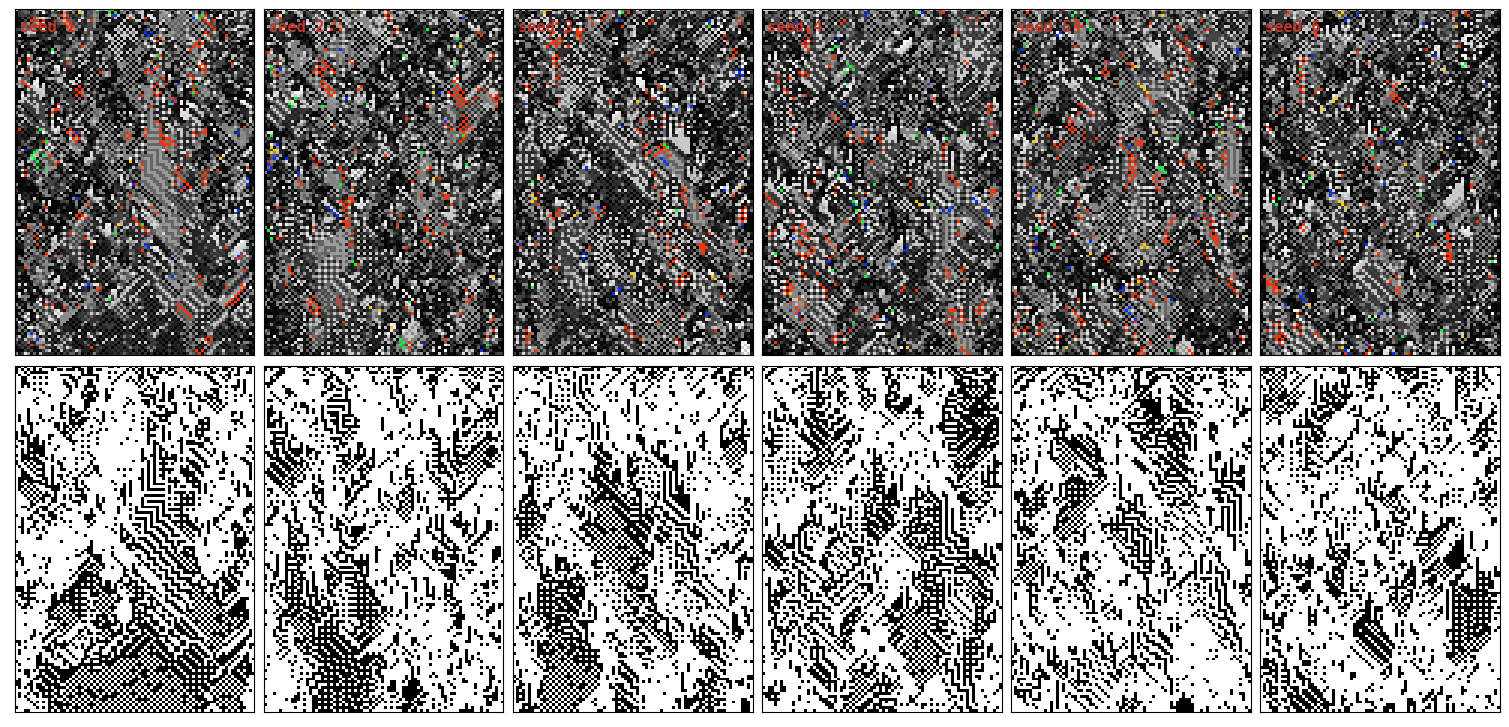
\includegraphics[width=\linewidth]{figures/river.png}
\caption{A \emph{river}: a composed operator sustains a reproducible
structure. The offset-$+2$ propagator, composed with a phenotype-reading,
four-candidate, first-match template construction (fallback: the all-zero
rule), produces in
each of six seeds a coherent band of alternating phenotype (bottom row)
drifting through a disordered background (genotype top, six seeds; genotype
coloured by rule as in Figures~\ref{fig:regimes}--\ref{fig:eoc}---greyscale by
byte value, with well-known ECAs highlighted, red~$=$~Rule~110). The band's
trajectory varies with the seed; its presence does not.
Where the bare rotations collapse or cycle (Figure~\ref{fig:eoc}), this
composition holds an off-critical structure for the length of the run.}
\label{fig:river}
\end{figure}

\section{Why Distance Geometry Cannot See This}
\label{sec:metrics}

The classification is a conjugacy invariant of the operator $\sig$---its
cycle type---while the complexity and compression measures we tried are
computed from a single rule's bits or from a single space--time trajectory. A
quantity read off one field's history does not have access to $\sig$'s cycle
type, so we should not expect it to recover the parity classification, and in
our tests it did not. The smallest surviving cast is small but not
degenerate---an all-even $\sig$ with a single $8$-cycle ($k=1$) has
$2^1 = 2$ fixed points, since a permutation of eight elements has at least one
cycle---yet a population-diversity count reads such a collapsed field as
nearly dead though it is maximally selected; a frozen periodic genotype scores
a lower statistical complexity $C_\mu$ \parencite{crutchfield1989inferring}
than Rule~110; gzip codelength rates a self-similar rule as noise. These
observables are not all metrics in the same sense, and we do not claim a
general impossibility theorem---only that the standard per-trajectory measures
we tried do not separate the parity classes, and that this is unsurprising
because the classifying property lives on the operator, not on the states.
The classification is a theorem \emph{because} it is not a per-trajectory
statistic.

\section{The Edge of Chaos, Locally}
\label{sec:discussion}

The survey of Figure~\ref{fig:eoc} exposes a sharp behavioural split within a
family of provably fixed-point-bearing operators: only offset $\pm 2$ sustains a
high-diversity, visually complex phase, while the rest collapse to near-uniform
fields. That surviving phase carries the visual signature long associated with
the \emph{edge of chaos} \parencite{langton1990computation}, and a reader is
entitled to ask whether the resemblance is more than skin deep. It is, but only
in a specific and measurable sense, and naming that sense is the purpose of this
section.

Two notions travel under the one phrase. The first is \emph{global}: a system
tuned by a control parameter to a critical point between an ordered and a
disordered phase---Langton's $\lambda$, which Section~\ref{sec:lambda} shows is
silent here, every fixed point sitting at $\lambda = 1/2$ by
Theorem~\ref{thm:lambda}. The second is \emph{local}: within a single
realisation, ordered and disordered regions coexist in space, and the edge of
chaos is the \emph{interface} between them---the domain walls of computational
mechanics \parencite{crutchfield1989inferring,shalizi2001computational}, where
structure propagates and interacts. It is the second that this object supports.

To expose the local structure we colour the genotype field not by rule identity
but by each rule's \emph{intrinsic dynamical character}: a scalar chaos score
obtained by running that rule alone as an elementary CA and measuring its
\emph{dynamical} activity---how much its field keeps changing over time, a
run-time quantity distinct from the static truth-table balance $\lambda$ of
Section~\ref{sec:lambda}. Ordered rules score near $0$; complex rules such as
Rule~$110$ near $0.4$; chaotic rules $0.5$ and above. Under this tint
(Figure~\ref{fig:tint}) the field resolves into coexisting domains of distinct
dynamical character---ordered, complex, and chaotic---separated by definite
boundaries rather than a uniform turbulence. Which regimes coexist depends on
the operator: offset $+2$ pairs ordered with chaotic, whereas
$\sigma = 16250374$ pairs ordered with the complex Rule~110 that comes to
dominate its field (\secref{sec:conclusion}). Thinning the boundary between
ordered and active regions to a filament skeleton recovers the ``separating
curve'' directly from the data.

The interface is not a clean line but a \emph{fractal}. Box-counting yields a
scale-free dimension (clean power laws, $R^2 > 0.99$) of $D \approx 1.5$ for
offset $+2$ and $D \approx 1.7$ for the phenotype-reading river of
Figure~\ref{fig:river}. Two features lift this above curiosity
(Figure~\ref{fig:interface}). First, across system sizes $L = 128$ to $768$ the
dimension \emph{stabilises} rather than drifting, and the coexistence fraction
is \emph{size-independent} ($\approx 0.4$ at every $L$): the operator neither
orders-out nor chaos-out as it grows, but holds a scale-invariant mixture.
Second, the behaviour cleanly separates sustaining from collapsing operators:
offset $+4$, superficially similar in isolation, loses its chaotic phase
\emph{entirely} at $L \ge 256$---the interface does not simplify, it disappears.
The edge of chaos, locally understood, is thus a persistent, scale-invariant
geometric feature of the sustaining operators and demonstrably absent from the
collapsing ones.

We deliberately stop short of two stronger claims. We do not assert a global
critical transition; consistent with Section~\ref{sec:limits}, the honest
reading remains a stable coexistence rather than a demonstrated critical point,
and the interface analysis here is exploratory---a handful of seeds, on the
fixed-boundary (line) variant rather than the wrapped lattice of
Figure~\ref{fig:eoc}; a boundary-matched, more heavily seeded finite-size
collapse is the natural next step. Nor do we claim computation: direct
injection--decode probes recover information storage and short-range
transmission on these fields, but no nonlinear modification under the conditions
tested. The edge of chaos we defend is the structural one---a scale-invariant
order/chaos interface---not the computational one.

The local picture also ties back to what makes these operators new. The
genotype--phenotype coupling is not incidental to the interface: the
phenotype-reading river sustains a \emph{denser} fractal boundary
($D \approx 1.7$) than the feedforward offset $+2$ ($D \approx 1.5$)---a
difference visible at the interface, though whether the coupling \emph{drives}
it we do not settle here. And it points at a sequel.
If the filaments are domain walls, they are candidate \emph{wires}: the natural
computational question is not which rules compose them---in our data the complex
rules are not enriched on the interface---but whether information is
\emph{transported along} them and \emph{combined where they collide}
\parencite{mitchell1993revisiting}. Whether computation flows down the
edge-of-chaos lines of these diagrams is, we think, a paper of its own.

\begin{figure}[tb]
\centering
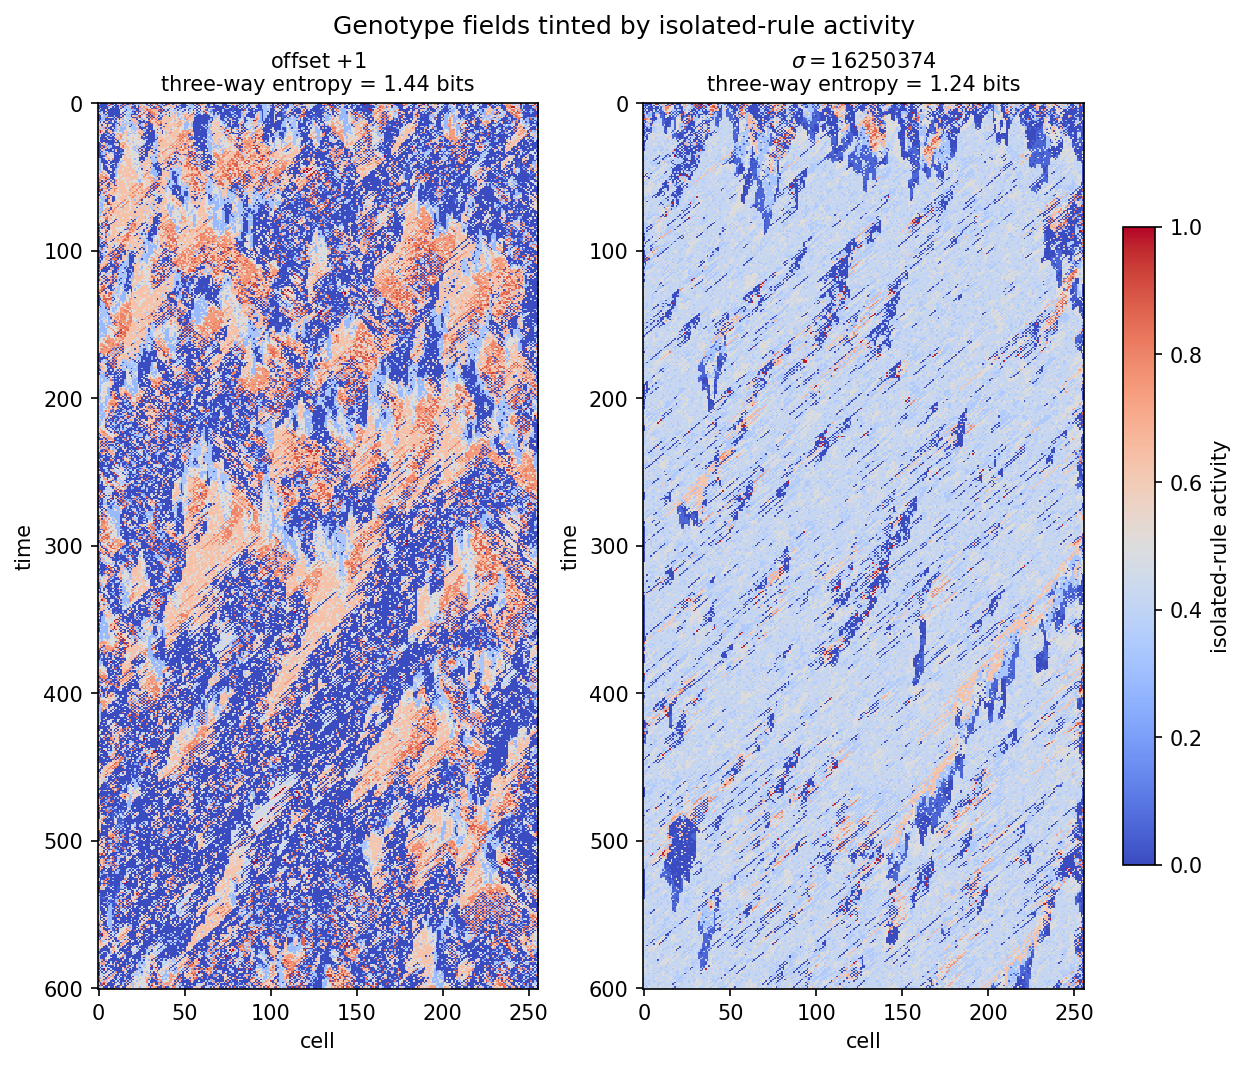
\includegraphics[width=0.68\linewidth]{figures/eoc_tint.png}
\caption{\textbf{The genotype as a map of dynamical regimes.} Genotype fields
(fixed-boundary variant) tinted by each rule's intrinsic chaos score---its
asymptotic activity as an isolated elementary CA (blue $=$ ordered near $0$,
pale $\approx$ complex near $0.4$, red $=$ chaotic near $0.5$ and above). The
field resolves into coexisting regimes, and which active regime pairs with the
ordered background depends on the operator: offset $+2$ mixes ordered and
genuinely \emph{chaotic} rules ($\approx 40\%$ chaotic at this seed), whereas
$\sigma = 16250374$ is dominated by the \emph{complex} Rule~110
($\approx 48\%$; Figure~\ref{fig:regimes}) and pairs ordered with complex. The
activity score orders the regimes but does not by itself separate complex from
chaotic, a known-hard distinction.}
\label{fig:tint}
\end{figure}

\begin{figure}[tb]
\centering
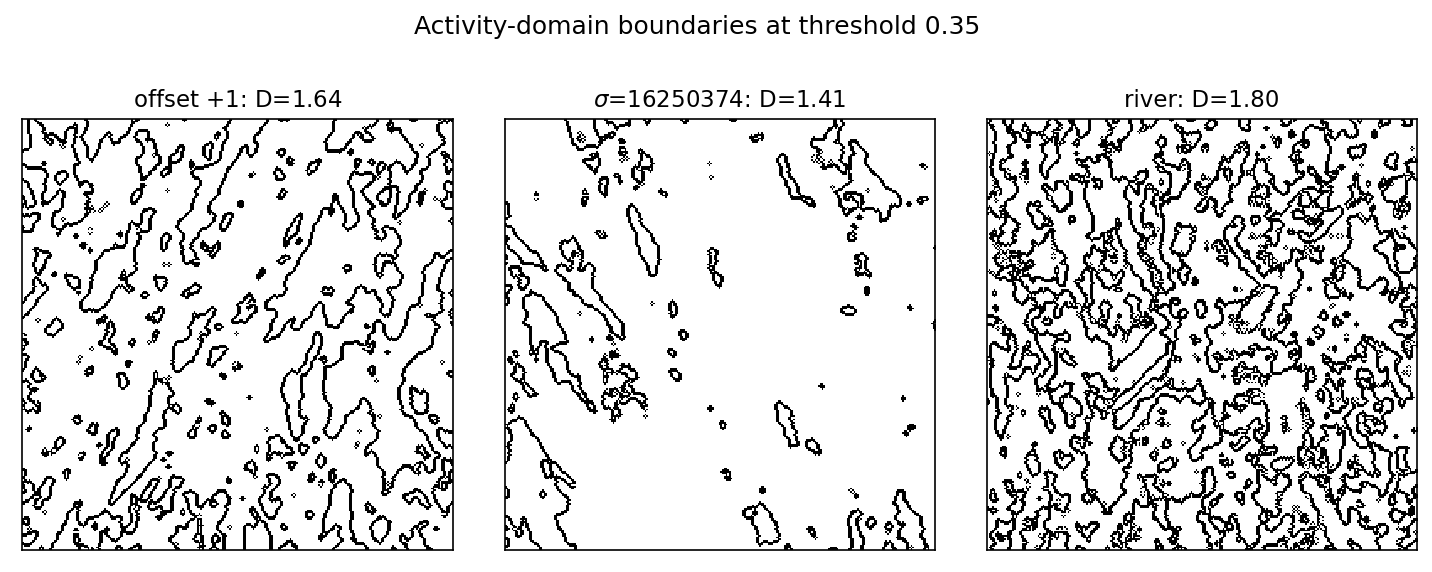
\includegraphics[width=\linewidth]{figures/eoc_interface.png}
\caption{\textbf{The order/chaos interface is fractal and size-stable for the
sustaining operators.} Top: the interface (black) extracted from the tinted
field at $L = 256$. offset $+2$ carries a coherent fractal boundary
($D \approx 1.53$); offset $+4$ has collapsed (no interface); the
phenotype-reading river carries a denser one ($D \approx 1.69$). Bottom:
box-counting dimension against system size $L$; the estimate stabilises rather
than drifting. Exploratory: a handful of seeds, fixed-boundary variant.}
\label{fig:interface}
\end{figure}

\section{Limits}
\label{sec:limits}

The theorems are the Boolean case and are exact; the dynamical claims are
narrower and empirical. The census and the sustained-diversity behaviour are
reported for a single spatial coupling ($S_8$, radius one, one value map) at
limited seed counts, and invite a fuller treatment; we use ``edge of chaos''
descriptively, not as a measured critical point. Section~\ref{sec:discussion}
takes up the local, structural reading and reports an exploratory
interface-dimension statistic under its own stated caveats (few seeds,
fixed-boundary variant); beyond it we report no perturbation-spreading or
entropy-rate statistics.
Because the dynamics is stochastic, every such figure is given both as a
fixed \emph{representative} seed and, where a scalar is quoted, as a fixed
\emph{six-seed sample} (mean and range); both are reproducible from the
pinned seeds through the accompanying package. The
substrate the object sits in is not itself new (\secref{sec:object}); $\lambda$
is one heuristic among several \parencite{wuensche1999classifying}, and we
make no claim that balance implies edge-of-chaos dynamics---only that here
balance is \emph{derived}. What is new, and what we rest the paper on, is the
object of Equation~\eqref{eq:prop} and the fixed-point structure that forces
every fixed rule to be balanced, $\lambda = 1/2$, as a matter of proof.

\section{Conclusion}
\label{sec:conclusion}

The characterisation promised at the outset (\secref{sec:object}) has two
halves. The
first is static and exact: which operators possess fixed points (the
all-even ones), how many ($2^k$), and where they lie (balanced,
$\lambda = 1/2$, always). The second is empirical and tentative. Because
every fixed point sits at $\lambda = 1/2$, that parameter is silent on the
difference between an operator whose field stays diverse and one whose field
collapses; the distinct-rule count is not, and in our
runs it separates the two across the rotation family by more than an order of
magnitude (Figure~\ref{fig:lambda}). The same observable offers a suggestive
reading of the search that produced the family, reported both as a
representative run and as a fixed six-seed sample (\secref{sec:limits}). The
operator of Figure~\ref{fig:regimes} that comes to be dominated by
Rule~110---a universal rule, the naive prize of a search for computational
intelligence---concentrates the field onto it and pays for it in diversity.
At the representative seed, $29\%$ of its genotype cells are Rule~110 and it
sustains $17$ distinct rules, against a foil that holds Rule~110 below $2\%$
and sustains $20$; over the six-seed sample the ordering is unchanged---Rule
110 $35\%$ (range $27$--$40\%$) versus $2\%$ ($1$--$2\%$), sustained diversity
$15$ versus $24$. On this pair, recovering a universal rule and sustaining a
diverse population pull against each other---a suggestion worth testing at
scale, not a law we have established.

\printbibliography
\end{document}
